\chapter{Meta}

\section{Vorgeschichte}

Wir sind leidenschaftliche Skateboarder und hatten anfangs Probleme damit, umliegende Parks
zu finden oder neue Skater-Kollegen kennenzulernen. Somit haben wir uns entschlossen eine
App bzw. eine Website zu entwickeln, die Anfängern das Leben erleichtern soll.

Durch die Funkion von \textbf{Skate-Buddy} Parks nach ihrer Nähe zu sortieren, ist es möglich
in Sekunden den naheliegendsten Park ausfindig zu machen. Außerdem wird die aktuelle Position
auf einer Map angezeigt, somit kann man also den schnellstmöglichen Weg ausfindig machen.

\section{Projektlogo}
\label{logo}

Auf dem Logo ist ein Skateboard zu sehen, welches durch ein Portal aus einem Smartphone fliegt.
Der Designer des Logos ließ sich vom Portal aus der Serie \textit{Rick and Morty} inspirieren und wollte damit die Verbindung zwischen
der Technik und dem Sport zum Ausdruck bringen.



\begin{figure}[H]
    \centering
    \hfill
    \subfigure[Rick and Morty Staffel 1 Werbebild~\cite{rickAndMortySeason1}]{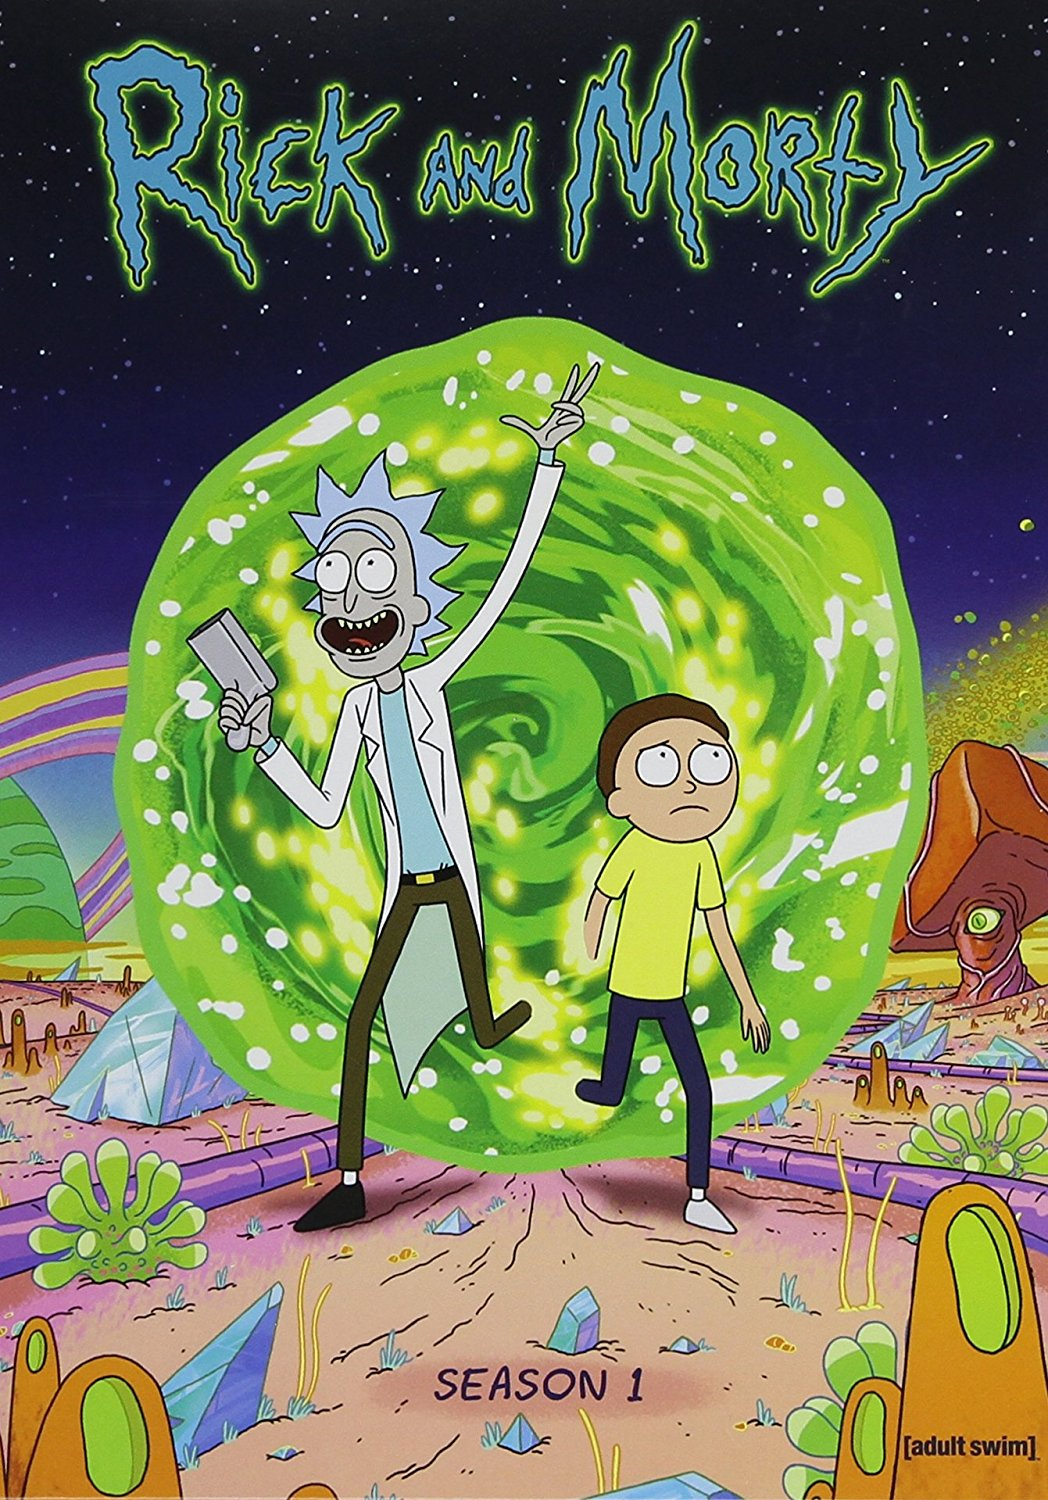
\includegraphics[height=0.4\textwidth]{images/Intro/RnM_S1.jpg}}
    \hfill
    \subfigure[SkateBuddy Projektlogo]{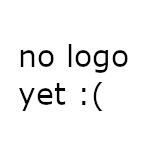
\includegraphics[width=0.4\textwidth]{images/logo.png}}
    \hfill
    \caption{Vergleich zwischen Portal aus der Serie und dem Logo}
\end{figure}